%%%%%%%%%%%%%%%%%%%%%%%%%%%%%%%%%%%%%%%%%%%%%%%%%%%%%%%%%%%%%%%%%%%%%%%%%%%%%%%%%%%%%%%%%%%%%%%%%%%%%%%%%%%%%
% % % % % % % % % % % % % % % % % % % % % % % % % % % % % % % % % % % % % % % % % % % % % % % % % % % % % % % 
% = = = = = = = = = = = = = = = = = = = = = = = = = = = = = = = = = = = = = = = = = = = = = = = = = = = = = =
%
% This is where the packages are declared

\documentclass[]{article}

\usepackage[english]{babel}
\usepackage[utf8]{inputenc}
\usepackage{amsmath}
\usepackage{amsthm}
\usepackage{dirtytalk}
\usepackage{bm}
\usepackage{subfig}
\usepackage{amsfonts}
\usepackage{graphicx}



\theoremstyle{definition}
\newtheorem{exmp}{Example}[section]

\begin{document}


\title{INFO 2301: Quantitative Reasoning for Information Science}
\author{Abe Handler \\ Department of Information Science \\ University of Colorado, Boulder}
\date{\today}

\maketitle

\begin{abstract}
An outline of what we've covered so far. You should be comfortable with everything in this document. 
\end{abstract}

\section{Sets}

A \textbf{set} is an unordered collection of items, without duplicates. 

People follow a number of conventions when talking about sets.

\begin{itemize}
    \item The items in a set are often called ``elements''
    \item We use capital letters to name sets
    \item We show the elements in a set using curly brackets
    \item A set can include any kind of element (e.g.\ strings, or kinds of apple)
\end{itemize}

\begin{exmp}
We can write the integers between 0 and 3 (including 0 and 3) as $A$ = $\{0,1,2,3\}$
\end{exmp}

\begin{exmp}
Because sets do not have order, if $ B= \{0,1\}$ and $C=\{1,0\}$, then $C=B$.
\end{exmp}

\begin{exmp}
A set of strings, $ P= \{ \text{\say{Denver},\say{Boulder},\say{Broomfield}} \}$
\end{exmp}

\begin{itemize}
    \item If $a$ is an element in $X$ then, we use the notation $a \in X$ 
    \item If $a \in X$ then we say that ``$a$ is in $X$''
    \item We write this: \verb|$a \in X$|
    \item If $a \notin X$ then we say that ``$a$ is not in $X$''
    \item We write this: \verb|$a \notin X$|
\end{itemize}

\begin{exmp}
Let $ C= \{1, 2\}$. Then $1 \in C$ and $6 \notin C$
\end{exmp}


\subsection{Subsets}

If all elements of $A$ are elements of $B$ then we say that $A$ is a subset of $B$.  We use the notation $ A \subset B$ (written \verb|$ A  \subset B $|) to indicate that $A$ is a subset of $B$.

\begin{exmp}\label{e:subset}
Let $ A= \{2, 1\}$ and $B = \{1,2,5\}$. Then $A \subset B$
\end{exmp}

In this class, when we use $ A \subset B$ we will assume that some elements of $B$ are not elements of $A$. So $A$ is a ``proper subset'' of $B$. For instance, in Example \ref{e:subset}, $A \subset B$ because $5 \in B$ and $5 \notin A$. If we want to allow for the possibility that $A=B$, we can use the notation $A \subseteq B$ (written \verb|$ A \subseteq B $|). 

\begin{exmp}
Let $ A= \{1, 2,3 \}$ and $B = \{1,2,3\}$. Then $A \subseteq B$ but not $A \subset B$
\end{exmp}

\begin{exmp}
Let $ A= \{1, 3 \}$ and $B = \{1,2,3\}$. Then $A \subseteq B$ and $A \subset B$
\end{exmp}

\subsection{Intersections, unions and complements}

\begin{itemize}

\item We use the notation $A \cap B$ (written \verb|$ A  \cap B $|) to indicate all of the elements that are in \textit{both} $A$ and $B$. This is called the \textit{intersection} of $A$ and $B$

\item We use the notation $A \cup B$ (written \verb|$ A  \cup B $|) to indicate all of the elements that are in $A$ or $B$. This is called the \textit{union} of $A$ and $B$.

\item To understand intersections and unions it is often helpful to draw venn diagrams. 

\end{itemize}

\begin{exmp}
Let $ A= \{1, 2, 3\}$ and $B = \{2,3,7\}$. Then $A \cap B$ = $\{2, 3\}$ and $A \cup B$ = $\{1,2, 3, 7\}$
\end{exmp}

\begin{itemize}
\item The complement of a set $A$ is the set of all elements that are not in $A$
\item The complement of a set requires defining $U$, the universal set of all possible elements
\item We write the complement of $A$ as $\overline{A}$ (written \verb|$ \overline{A} $| 
\item We can also write the complement as $A^c$  (written \verb|$ A^c $|)
\end{itemize}

\begin{exmp}
Let $ U= \{1, 2, 3\}$ and $A = \{2\}$. Then $\overline{A}$ = $\{1, 3\}$ 
\end{exmp}

\subsection{Cardinality}

The number of items in a set is called the \textit{cardinality} of the set. We use the notation $\vert F \vert$ (written \verb|$ \vert F \vert $|) to indicate the cardinality of a set.

\begin{exmp}
Let $ F = \{1, -2, 42 \}$, then $\vert F \vert$ = 3
\end{exmp}

\textit{If you spot any errors in this document, or if anything is needlessly confusing, please send me an email. I will assign extra credit.}

\section{Functions}

\begin{itemize}
\item A function maps elements from one set to another. 
\item The first set is called the domain.
\item The second set is called the range. 
\item A function maps each element from the domain to exactly one element in the range.
\item We write this $f: A \rightarrow B$ where $f$ is a function mapping elements of $A$ to $B$ (written \verb|$f: A \rightarrow B $|) 
\end{itemize}

\begin{exmp}
Let $A$ be a set $\{0,1,2,3\}$ and let $f$ be a function mapping every element of $A$ to -19. The domain of $f$ is $A$ and the range is $\{-19\}$
\end{exmp}

\begin{exmp}
Let $A$ be the set of all integers and let $B$ be the set of all integers. The \texttt{addOne} function maps each element in $A$ to the element in $B$ that is exactly one greater. For instance, the \texttt{addOne} function maps 4 to 5.
\end{exmp}

\section{Vectors}

\begin{itemize}
\item A vector is a list of numbers. 
\item Each number in the vector is called a ``component'' and represents a dimension of the vector. 
\item We denote vectors with bold, lower-case letters and triangle brackets, such as $ \mathbf{x}=<1,2> $ (written \verb|$  \mathbf{x}=<1,2> $|)
\item We can use subscripts to refer to components of a vector. If $\mathbf{x}=<6,9>$ then $\mathbf{x}_1$ = 6 (assuming indexing starting at one)
\end{itemize}

\subsection{Vector addition}

Vector addition is an operation which takes two input vectors and returns one output vector. If  $\mathbf{x}=<x_1, x_2 ... x_n>$ and $\mathbf{y}=<y_1, y_2 ... y_n>$  then  $\mathbf{x}+\mathbf{y}=<x_1 + y_1, x_2 + y_2 ... x_n + y_n>$.

\begin{exmp}
$\mathbf{x}=<3,4>$ and $\mathbf{y}=<-1,2>$  then  $\mathbf{x}+\mathbf{y}=<2,6>$
\end{exmp}

\subsection{Summation notation}

Summation notation is important for vector operations, and in many other areas of math. 

\begin{itemize}
\item To indicate the sum of a sequence of items, we write $\Sigma_{i=0}^Nx_i$ where $x_i$ is the $i$th item in a sequence. 
\item You can read this as summing over a sequence of items, from item 0 to item $N$. 
\item You can think of $i$ as an index into the sequence, in the same way you may think of $i$ as an index into an array. 
\item Usually, in 2301, the sequence being indexed is positive integers: 1,2,3,4 ... etc. So $x_1$ is usually 1, $x_2$ is usually 2, etc. You can assume we are indexing into the positive integers unless otherwise specified.
\item We write sigma notation in \LaTeX~as \verb|$ \Sigma_i=0^Nx_i $|
\end{itemize}

\begin{exmp}
You can also use summation notation without indexing into a sequence, e.g.\ $\Sigma_{n=1}^{N=3} (n+1) = (1+1) + (2+1) + (3 + 1) = 2 + 3 + 4$.
\end{exmp}

You can also use this notation to describe the sum of items in a sequence, after applying some operation.

\begin{exmp}
If $x=[1,2,3,4,5]$ then $\Sigma^5_{i=1} x_i^2 = 1^2 + 2^2 + 3^2 + 4^2 + 5^2 = 1 + 4 + 9 + 16 + 25 = 55$
\end{exmp}

\begin{exmp}
Note that you should read the $i$ as indexing into an array. So if you have an array $x=[2,3,4]$ then $\Sigma^3_{i=1} x_i = x_1 + x_2 + x_3 = 2 + 3 + 4$
\end{exmp}


\subsection{Euclidean norm}

The Euclidean norm of a vector is  $\vert \vert x \vert \vert_2$ = $\sqrt{\Sigma_{i=1}^{N} x_i ^2}$. You can think of the Euclidean norm as the size of a vector. 
\begin{exmp}
If $ \mathbf{x}=<-2,2> $ then  $\vert \vert x \vert \vert_2$ = $\sqrt{-2^2 + 2^2} = \sqrt{4 + 4}  = \sqrt{8}$  
\end{exmp}

\noindent Note: There are also other norms, which offer other ways of defining the size of a vector.

\subsection{Normalizing a vector}

\begin{itemize}
\item To normalize a vector, divide each component by the (Euclidean) norm. This creates a new ``unit vector'' with a norm of 1. 
\item People sometimes write unit vectors with ``hats'' over them, e.g.  $\hat{\bm{b}}$ (written \verb|$ \hat{\boldsymbol{b}} $|, where \verb|$ \boldsymbol $| means to write the symbol in bold).
\end{itemize}

\begin{exmp}
If $ \mathbf{x}=<-2,2> $ then  $\vert \vert x \vert \vert_2$ = $\sqrt{-2^2 + 2^2} = \sqrt{4 + 4}  = \sqrt{8}$. The unit vector of $ \mathbf{x}$ is $ \mathbf{\hat{x}}=<\frac{-2}{\sqrt{8}},\frac{2}{\sqrt{8}}> $. The Euclidean norm of the unit vector is $\sqrt{(\frac{-2}{\sqrt{8}})^2 + (\frac{2}{\sqrt{8}})^2}$ = $\sqrt{\frac{4}{8} + \frac{4}{8}}$ = $1$, so you know you have a unit vector. 
\end{exmp}

\subsubsection{You can normalize any vector}
Any vector can be converted into a unit vector. Here is an argument for this claim in 2D. It is easy to extend to any dimension. It is OK to skip this part if you want to just trust that you can always normalize. Assume we have a Euclidean norm of $N$. The following is true by definition in 2D.

\begin{equation}
a^2 + b^2 = N^2 
\end{equation}

Divide each side by $N^2$

\begin{equation}
\frac{a^2}{N^2} + \frac{b^2}{N^2} = 1
\end{equation}

Take the root of each side

\begin{equation}
\sqrt{\frac{a^2}{N^2} + \frac{b^2}{N^2}} = \sqrt{1}
\end{equation}

Simplify, recalling that the square root of 1 is 1.

\begin{equation}
\sqrt{(\frac{a}{N})^2 + (\frac{b}{N})^2} = 1
\end{equation}

Therefore, by definition, if you divide each component by $N$ you get a normalized vector.

\subsection{Dot product}

There are two ways to think about the dot product. You can think about it geometrically (in pictures) or algebraically (in symbols). It's better to build geometric intuition than to plug and chug through the algebraic version, but both are important to know really well.

\begin{itemize}
\item Algebraically, the dot product is defined as $\bm{a} \cdot \bm{b}$  = $\sum_i \bm{a}_i \bm{b}_i$.
\item Geometrically, the dot product is defined as $\bm{a} \cdot \bm{b}$  = $ \vert\vert  \bm{a}  \vert\vert \text{ }   \vert\vert  \bm{b}  \vert\vert \text{ }  \text{cos }  \theta $. This follows from the fact that the dot product between two vectors $\bm{a} \cdot \bm{b}$ (the dot symbol is written \verb|$ \cdot $|) is defined as the projection of $\bm{a}$ onto $\hat{\bm{b}}$, the unit vector of $\bm{b}$. (The lecture included a brief derivation.) You can think of the projection as the shadow $\bm{a}$ casts onto $\hat{\bm{b}}$. Another way to think about the dot product is the extent to which $\bm{a}$ and $\bm{b}$ point in the same direction, given that they might have different sizes (norms).
When the angle between the vectors is acute, the dot product is positive. When it is obtuse the dot product is negative.
\end{itemize}

\begin{figure}[h]
     \centering
     \subfloat[][a]{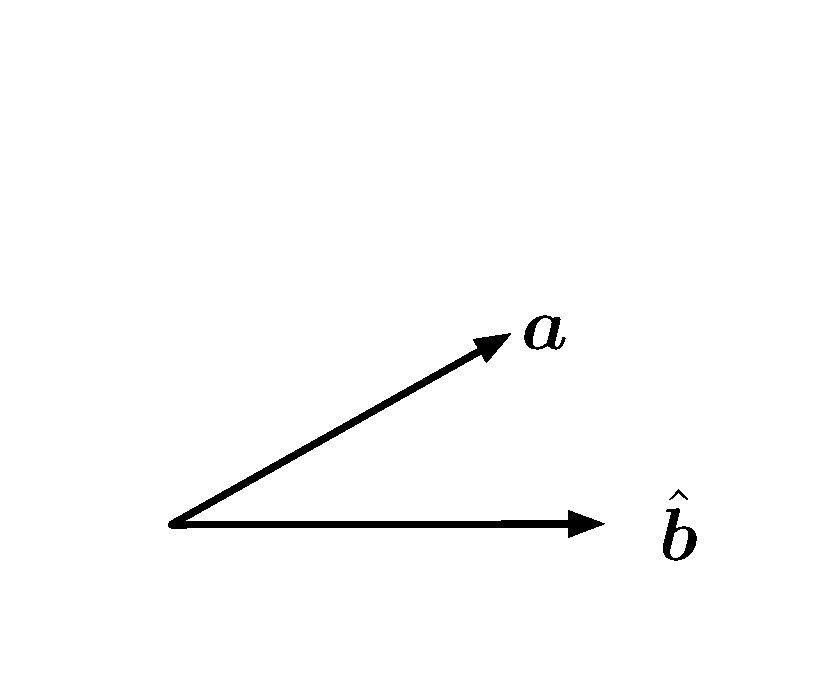
\includegraphics[width=3cm]{dot_prod_acute}\label{<figure1>}}
     \subfloat[][b]{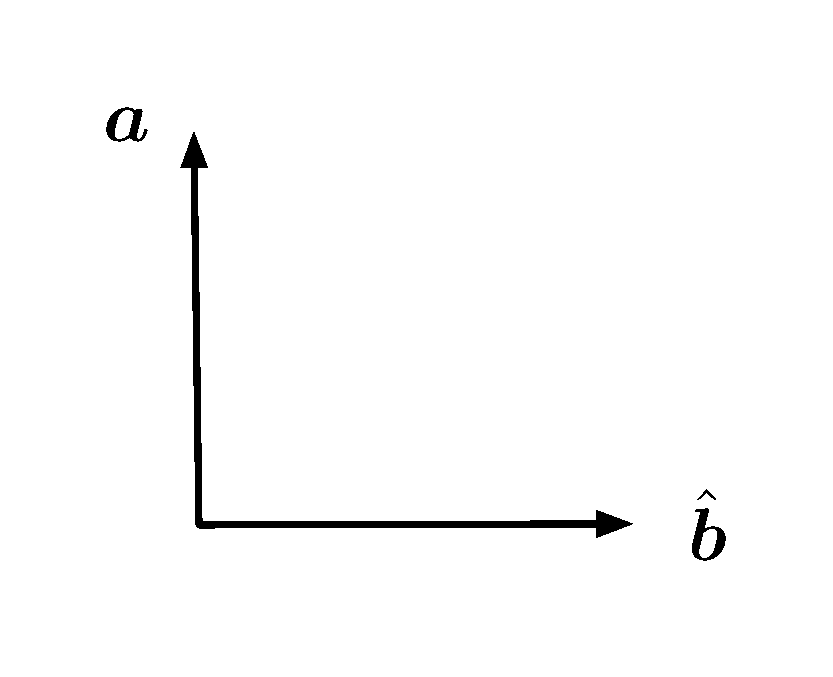
\includegraphics[width=3cm]{dot_prod_perp}\label{<figure2>}}
     \subfloat[][b]{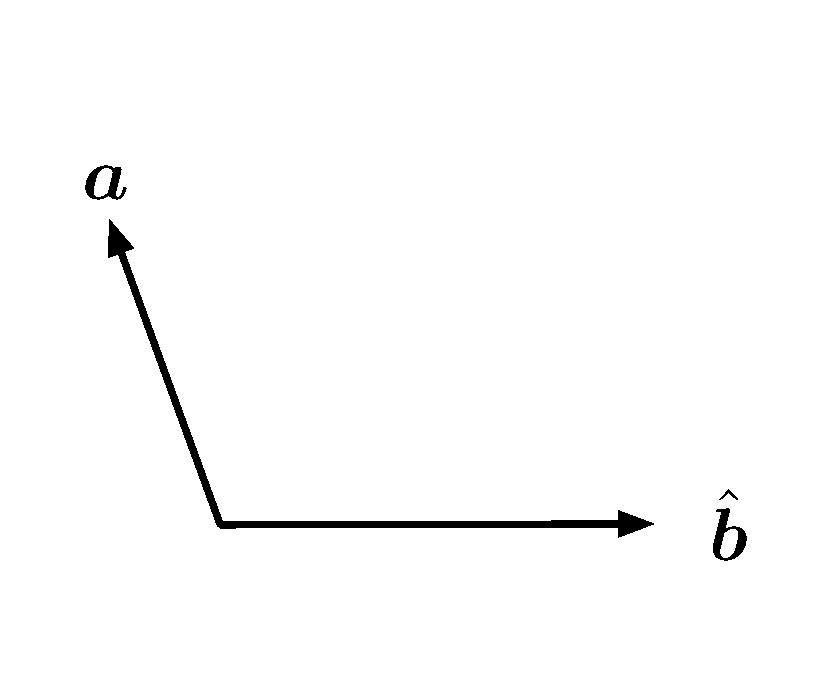
\includegraphics[width=3cm]{dot_prod_oblique}\label{<figure2>}}
     \caption{The dot product is positive when the angle $\theta$ between $\bm{a}$  and $\hat{\bm{b}}$ is less than 90 degrees (left). It is zero when $\theta$ = $90^{\circ}$. It is negative when $\theta$ is greater than  $90^{\circ}$.}
     \label{steady_state}
\end{figure}

\begin{exmp}
If $ \mathbf{x}=<-2,2> $ and then $ \mathbf{y}=<-1,7> $ then $\bm{x} \cdot \bm{y}$ =  $\sum_i \bm{x}_i \bm{y}_i$ = $-2 * -1 + 2 * 7$ = 2 + 14 = 16
\end{exmp}

\section{Booleans}

A Boolean variable can take on the value True or False. A Boolean expression is a collection of Boolean variables, joined by logical operators.

\subsection{NOT}

The simplest Boolean operator is NOT. The NOT operator takes a single Boolean operand. It flips the value of the Boolean variable (so True becomes False, and vice versa.) For instance, $A$ might be Boolean variable equal to True. Then NOT A is False. We also write this as $\neg A$ (\verb|$ \neg $|).

\subsection{AND}
The Boolean operator AND takes two Boolean variables as operands. The operator returns True if both variables are True. We write this $ A \wedge B$ (\verb|$ A \wedge B $|)

\subsection{OR}
The Boolean operator OR takes two Boolean variables as operands. The operator returns True if either variables is True. We write this $ A \vee B$ (\verb|$ A \ve B $|)

\begin{exmp}
If $A$=True and $B$=True then  $ A \wedge B$ is True
\end{exmp}

\begin{exmp}
If $A$=True and $B$=False then  $ A \wedge B$ is False
\end{exmp}

\begin{exmp}
If $A$=True and $B$=False then  $ A \vee B$ is False
\end{exmp}

\begin{exmp}
If $A$=True and $B$=False then  $ A \wedge \neg B$ is True because $\neg B$ is True and the AND of two true variables is True
\end{exmp}

\subsection{Evaluation}

Evaluating a Boolean expression means determining if the expression is True or False, based on the values of its variables. To evaluate a Boolean expression you should fill in the value of each variable and simplify.

\begin{exmp}
If $A$=True and $B$=False and $C$=True then  $ (A \vee B) \wedge C$ = $ (T \vee F) \wedge T$ = $ T \wedge T = T$  
\end{exmp}

\section{Probability}

\subsection{The sample space}

The sample space $\Omega$  (written \verb|$\Omega$|) is the set of all outcomes of an experiment. An event $A$ is a subset of the sample space. 

\begin{exmp}
If we toss a coin twice then $\Omega$=$\{HH, HT, TH, TT\}$
\end{exmp}

\begin{exmp}
If we toss a coin twice then $\Omega$=$\{HH, HT, TH, TT\}.$ The event ``at least one tails'' is $A=\{HT, TH, TT\}$. Notice that $A \subset \Omega$.
\end{exmp}

\subsection{Probability distribution}

A probability distribution is a function that maps events to real numbers between 0 and 1, and that satisfies the following three properties

\begin{itemize}
\item $p(A) \geq 0$ for all $A$
\item $p(\Omega) = 1$
\item If $A$ and $A^\prime$ are disjoint (i.e. their intersection is $\emptyset$) then $p(A \cup A^{\prime}) =  p(A) + p(A^{\prime})$
\end{itemize}

\begin{figure}[h]
     \centering
    	{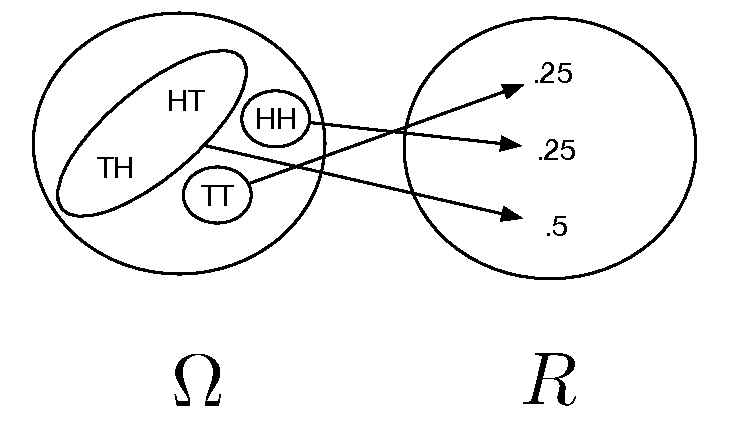
\includegraphics[width=5cm]{prob_distro}}
    \caption{An experiment flipping a fair coin twice. This probability distribution maps three events in $\Omega$ to a number between 0 and 1.}
     \label{steady_state}
\end{figure}

There are two interpretations of a probability distribution

\begin{itemize}
\item In the long run, if you keep running an experiment, the probability of a given event $A$ is the fraction of times you observe $A$, among all times you run the experiment. For instance, if you keep flipping a fair coin forever, you should expect that, in the long run, half of the time you will get heads. This is sometimes called the \textbf{frequentist} interpretation. 
\item Another interpretation of a probability distribution is that the distribution reflects your subjective belief about what will happen if you run an experiment in the future. For instance, if you believe (based on observing data) that you will get heads about half of the time the fact that $p(H)=.5$ (i.e.\ the probability of heads is 50\%) reflects your belief that about what will happen if you flip a coin. This perspective is sometimes called the \textbf{Bayesian} interpretation.
\end{itemize}

\subsection{The uniform distribution}

If all events are equally probable, we say that the distribution is uniform. If a distribution is uniform, then probability of any event $A \subset \Omega$ is $p(A)=\frac{1}{\vert \Omega \vert}$.

\begin{exmp}
If you roll a fair 6-sided die, all outcomes are equally likely so the distribution over outcomes is uniform. The probability of the event 1 is $p(\{1\})=\frac{1}{\vert \Omega \vert}$ = $\frac{1}{6}$.
\end{exmp}

\subsection{Determining a distribution from data (aka ``learning'')}

In the previous examples, we have largely known how the data was generated. For instance, we know that a fair die will land on the number 3 roughly $\frac{1}{6}$ of the time (if we keep rolling the die forever). But usually in nature you \textit{don't} know how the data was generated. You just see data and you have to make an educated guess about how it was created. 

If you have heard people mentioning \textbf{machine learning}, part of what they are talking about is a set of computational methods for reasoning about an (unobserved) probability distribution from observed data. Outside of computer science, you will also hear the process of reasoning about an unobserved distribution from data described as \textbf{statistical inference}.

\begin{exmp}
For example, say you observe 10 flips of a coin and get TTTTTHTTTT. Based on this data, do you think the probability distribution (i.e.\ the long run probabilities of getting heads or tails) is uniform? Well, there are two outcomes $\Omega=\{$H, T$\}$. If a distribution is uniform then we should expect that $p($H$) = \frac{1}{\vert \Omega \vert} =  \frac{1}{2}$ and $p($T$) = \frac{1}{\vert \Omega \vert} = \frac{1}{2}$. 

In this example, in the observed data there are 10 flips and only 1 heads. It is possible to get 9 out of 10 tails from a fair coin, but it is really unlikely. So you might make an educated guess that $p($H$) \neq \frac{1}{2}$ and that the distribution is not uniform. If you were to keep flipping the coin 10,000 times and see that only 1 out of 10 flips is heads, you can be pretty confident (but not totally certain) that the distribution is not uniform. 
\end{exmp}

\subsection{Independence}

Two events $A$ and $B$ are independent if $P(A \cap B)$ = $P(A)P(B)$. Intuitively, if the outcome of $A$ does not affect the outcome of $B$ then $A$ and $B$ are independent. 

\begin{exmp}
If you flip a coin twice, then the value of the first flip does not effect the value of the second flip. Thus the flips are independent.
\end{exmp} 

\begin{exmp}
On the other hand, your height and weight are likely not independent; if you are a taller person you likely have a larger weight than a shorter person. We say that these events are dependent (i.e.\ not independent).
\end{exmp} 

\begin{exmp}
Let's say we toss a fair coin five times. What is the probability of getting at least 1 head? Well, because probability sums to 1, the probability of at least one head is 1 minus the probability of all tails. If the fail flips are independent, then this is 1 minus the probability of tails on the first flip times the probability of tails on the second flip times the probability of tails on the third flip. 
\end{exmp}

\subsection{Conditional probability}

\begin{itemize}
\item The conditional probability of event $A$ is the probability of observing event $A$ given that you observed event $B$. 

\item We write conditional probability using the notation $p(A|B)$ (i.e.\ \verb|$ p(A \vert B) $|). You should read this as the probability of $A$ given $B$.

\item Formally, $p(A \vert B) = \frac{p(A \cap B)}{p(B)}$
\end{itemize}


\begin{exmp}
For instance, in general, taller people tend to weigh more than shorter people. So if you know that someone weighs over 200 pounds, it's more likely that they will be over 6 feet tall (compared to a person who weighs less than 200 pounds). Thus, the probability of observing event $A$ (i.e.\ a person who is over 6 feet tall) is higher if you first observe event $B$ (i.e.\ observing a person who weighs more than 200 pounds).
\end{exmp}

\begin{figure}[h!]%
    \centering
    \subfloat[\centering The probability of observing two tails on two flips is .25]{{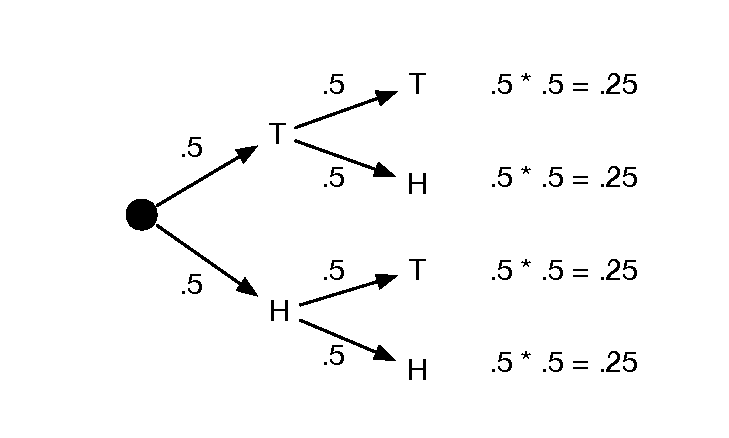
\includegraphics[width=5cm]{not_condition_onA.pdf} }}%
    \qquad
    \subfloat[\centering The probability of observing two tails, given that the first flip is T is .5]{{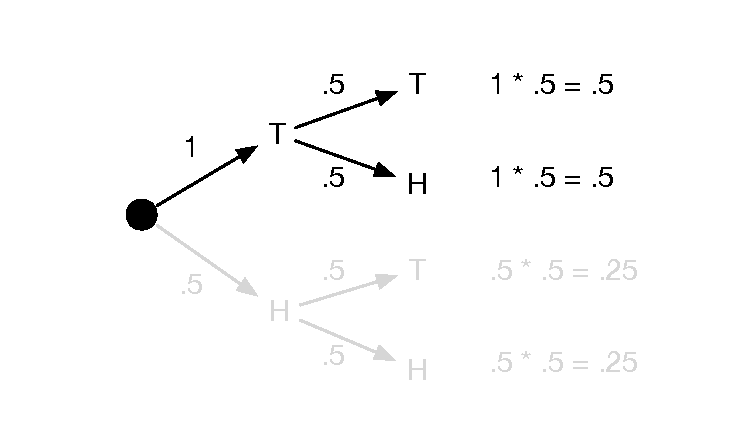
\includegraphics[width=5cm]{conditioned_onA.pdf} }}%
    \caption{Probability of getting two tails on two flips of a fair coin. Note that the events are independent so $p($T $ \cap $ T$)$ $= p($T$)$p$($T$)$ and  p$($T $\vert$ T$)=$p$($T$)$}%
    \label{fig:example}%
\end{figure}

\subsubsection{Independence revisited, after conditional probability} 

Intuitively, if two events $A$ and $B$ are independent, then the value of $A$ does not affect the value of $B$. We can reconsider independence in light of conditional probability. $p(B|A)$ gives the probability of $B$ given $A$. If $A$ and $B$ are independent then we should not expect the value of $B$ to depend on $B$. We can show this in the math. 

By definition:

\begin{equation}
p(B|A) = \frac{p(B \cap A)}{p(A)}
\end{equation}

If $B$ and $A$ are independent, then $p(B \cap A) = p(B)p(A)$. Thus we can rewrite the above:

\begin{equation}
p(B|A) = \frac{p(B)p(A)}{p(A)}
\end{equation}

The $p(A)$ terms cancel (these just represent numbers after all) so \underline{if} $A$ and $B$ are independent we have:

\begin{equation}
p(B|A) = p(B)
\end{equation}

Note that this is \underline{NOT} true if $A$ and $B$ are dependent (i.e.\ not independent).

\subsection{Random variables}

A random variable $X: \Omega \rightarrow \mathbb{R}$ is a function that maps each element in the sample space to a real number. Sometimes we abbreviate random variables as ``r.v."

\begin{exmp}
If you flip a coin twice, then $\Omega = \{HH, HT, TH, TT\}$. Let $X$ be a r.v.\ equal to the number of heads in a sequence. Thus $X$ maps $HH$ to the number 2. $X$ maps $TT$ to the number 0.
\end{exmp} 

\subsection{Expected value}

The expected value of a random variable $X$ is the average value you would expect the variable $X$ to take. We write the expected value as $E[X]$. Intuitively, you can think of the expected value as what you should expect the value of $X$ to be. Formally, for a discrete r.v.\ (we will only focus on discrete variables in this class) the definition is: 

\begin{equation}
E[X] = \Sigma^X p(x_i) * x_i
\end{equation}

\noindent where $p(x_i)$ is the probability of some outcome and $x_i$ is the value of that outcome.

\begin{exmp}
A friend offers to bet on the Broncos game on Sunday. If the Broncos win, you get \$100. If the Broncos lose, you pay \$50. Say that based on the last three years of Broncos games there is a 25\% chance the Broncos win and a 75\% chance the Broncos lose. The expected value of the proposed bet is .25 * -50 + .75 * 100 = 62.5. You should take the bet because you should expect to win \$62.5.
\end{exmp} 

\subsection{Variance}
Some random variables take values that are spread out. Other random variables take values in a narrower range.

\begin{exmp}
House cats usually way between 5 and 20 pounds. Pet dogs usually weigh between 10 and 100 pounds. Say you have a sample of pet cats and dogs. If $X$ is a r.v.\ that maps a dog in a sample to its weight, and $Y$ is an r.v.\ that maps a cat in a sample to its weight, then $X$ is more spread out than $Y$.
\end{exmp} 

\begin{itemize}
\item The variance offers a way to quantify how spread out a variable is. 
\item A variance is an expected value. 
\item Specifically, it is the expected value of how far a variable is from the mean.
\item Formally, the variance of a discrete r.v.\ is $Var[X]=E[(X - E[X])^2] = \sum p(x_i) (X - E[x])^2$
\item The standard deviation $\sigma$ is the square root of the variance
	\begin{itemize}
	\item[] i.e.\ $\sqrt{Var(X)}=\sigma$
 	\end{itemize}
\end{itemize}

\begin{exmp}
You flip a coin twice. Let $X$ be a r.v.\ mapping to the number of heads across two tosses. The sample space is $\Omega=\{HH,HT,TH,HH\}$ and $p(X) = \frac{1}{4}$. Recall that the r.v.\ $X$ is a function. So, for instance, $X(HH)=2$ and $X(HT)=1$. 
\begin{itemize}
\item Let's start by computing the expected value, which we need to calculate the variance. By definition, we get the following:
	\begin{itemize}
	\item[] $E[X] = \sum p(HH)X(HH) + p(HT)X(HT) +  p(TH)X(TH) + p(TT)X(TT)$
	\end{itemize}
\item If we plug in numbers for probabilities we get the following:
  \begin{itemize}
    \item[] $E[X] = \sum \frac{1}{4} X(HH) + \frac{1}{4} X(HT) +\frac{1}{4} X(TH)+ \frac{1}{4} X(TT)$
   \end{itemize}
\item If we plug in numbers for values of $X$ we get the following:
  \begin{itemize}
	\item[] $E[X] = \sum \frac{1}{4} * 2 + \frac{1}{4} * 1 +\frac{1}{4}* 1 + \frac{1}{4} * 0$
   \end{itemize}
\item If we simplify we get the following:
  	\begin{itemize}
		\item[] $E[X] = \sum \frac{2}{4} + \frac{1}{4} +\frac{1}{4} + 0 = 1$
	\end{itemize}
\item Thus $E[X]=1$, meaning that if we flip a coin twice, on average, we will get 1 head.
\item Now that we know $E[X]$ we can ask: what is the variance? We start by applying the definition.
\item $Var[X] = \sum p(x_i) (X - E[x])^2$
\item Thus... 
\item $Var[X] = \sum p(HH)(X(HH) -1)^2 + p(HT)(X(HT) -1)^2 +  p(TH)(X(TH) -1)^2 + p(TT)(X(TT) -1)^2$
\item If we plug in numbers for probabilities we get the following:
  \begin{itemize}
    \item[] $Var[X] =  \sum \frac{1}{4} (X(HH) -1)^2 +  \frac{1}{4} (X(HT) -1)^2 +   \frac{1}{4}(X(TH) -1)^2 +  \frac{1}{4}(X(TT) -1)^2$
   \end{itemize}
\item If we plug in values for random variables, we get the following: 
  \begin{itemize}
   \item[] $Var[X] =  \sum \frac{1}{4} (2 -1)^2 +  \frac{1}{4} (1 -1)^2 +   \frac{1}{4}(1 -1)^2 +  \frac{1}{4}(0 -1)^2$
   \end{itemize}
\item If we simplify we get the following:
 	 \begin{itemize}
   	\item[] $Var[X] =  \sum \frac{1}{4} (1)^2 +  \frac{1}{4} (0)^2 +   \frac{1}{4}(0)^2 +  \frac{1}{4}(-1)^2$
   	\item[] $Var[X] =  \sum \frac{1}{4} * 1 +  \frac{1}{4} * 1$
   	\item[] $Var[X] = \frac{1}{2}$
   	\end{itemize}
\item The expected squared deviation from the mean (i.e.\ the variance) is $\frac{1}{2}$. This is a quantitative measure of how spread out $X$ is.
\end{itemize}

\end{exmp} 

\subsection{Bayes rule}

Bayes rule tells you the probabilty of some event $B$, given that you know that some other event $A$ has happened. Usually when you apply Bayes rule you know how to compute $p(A|B)$ but not $p(B|A)$. Thus you apply the law of conditional probability like this: 

\begin{align*}
p(B \vert A) &= \frac{p(B \cap A)}{p(A)} && \text{law of conditional probability} \\
       &= \frac{p(A \vert B)p(B)}{p(A)} && \text{via multiplication law}
\end{align*}

\noindent this gives Bayes rule $p(B \vert A) = \frac{p(A \vert B)p(B)}{p(A)}$. Note that $p(A) = \sum p(A|B^\prime)p(B^\prime)$, by the law of total probability. To remember Bayes rule, it helps to think of ``flipping the conditional'' from $p(A \vert B)$ to $p(B \vert A)$. 


\textbf{Note:} In Bayesian statistics, the terms on the right have special names. $p(A)$ is called the \textit{evidence}, $p(A \vert B)$ is called the \textit{likelihood} and $p(B)$ is called the \textit{prior}. 

\end{document}